% 02_chinese.tex
\chapter{遭遇中文}
\label{chap:chinese}

如果你有认真做第~\ref{chap:hello_world}~章的额外习题,那么你很可能已经发现,
使用 \lstinline[style = iltx]|article| 等\emph{标准文档类}无法在 PDF 文件
中打印中文。今次我们来解决这个问题。

\section{代码和解释}

\begin{lstlisting}[style = lltx, caption = {你好 \LaTeX{}}, label = {lst:chinese}]
\documentclass[UTF8, a4paper, zihao = -4]{ctexart}
\title{第一篇中文手稿}
\author{孟晨}
\date{\today}
\begin{document}
\maketitle
% 这是注释

你好 \LaTeX!我有一个质能方程:$E = mc^2$。
\end{document}
\end{lstlisting}

这份代码和第~\ref{chap:hello_world}~章的代码相似度有 9 分,应该是比较好看懂的。
这里对不同之处做一些解释。

首先是载入文档类的地方,之前载入的是 \lstinline[style = iltx]|article|,
现在载入的是 \lstinline[style = iltx]|ctexart|。这是 \ctex{} 宏集提供的文档类,
用于在 \lstinline[style = iltx]|article| 的基础上提供中文支持和中文版式支持。
与之类似的,还有 \lstinline[style = iltx]|ctexbook| 和
\lstinline[style = iltx]|ctexrep|。它们分别是 \lstinline[style = iltx]|book| 和
\lstinline[style = iltx]|report| 的汉化版。

\lstinline[style = iltx]|ctexart| 是 \lstinline[style = iltx]|article| 的升级版。
因此,\lstinline[style = iltx]|ctexart| 支持 \lstinline[style = iltx]|article| 的
所有参数;并且在 \lstinline[style = iltx]|article| 的基础上有所扩充。
扩充的 \lstinline[style = iltx]|UTF8| 参数,告诉 \ctex{} 宏集,
我们这篇文稿使用 UTF-8 编码。扩充的 \lstinline[style = iltx]|zihao = -4| 参数,
则告诉 \ctex{} 宏集,我们这篇文稿使用小四号字(取代 \lstinline[style = iltx]|12pt|)。

\begin{warning}
  如果没有明确的理由,请不要使用 \pkg{CJK} 宏包。这是一个过时的宏包,并且在中文处理上
  存在很多的问题。

  如果没有明确的理由,也请不要单独使用 \pkg{xeCJK} 宏包。它只解决了中文支持的问题,却没有
  解决中文版式处理的问题。\ctex{} 宏集在使用 \XeLaTeX 时会自动调用 \pkg{xeCJK} 宏包。
\end{warning}

\section{操作和输出}

请将代码清单 \ref{lst:chinese} 中的内容,用键盘逐字母地输入进电脑,
并保存在文件 \file{02\_chinese.tex} 中。注意,请将文件以 UTF-8 编码保存。
点击「排版」,以 \XeLaTeX{} 编译,你应该看到如图 \ref{fig:chinese} 所示的样子。

\begin{figure}[!htb]
\centering
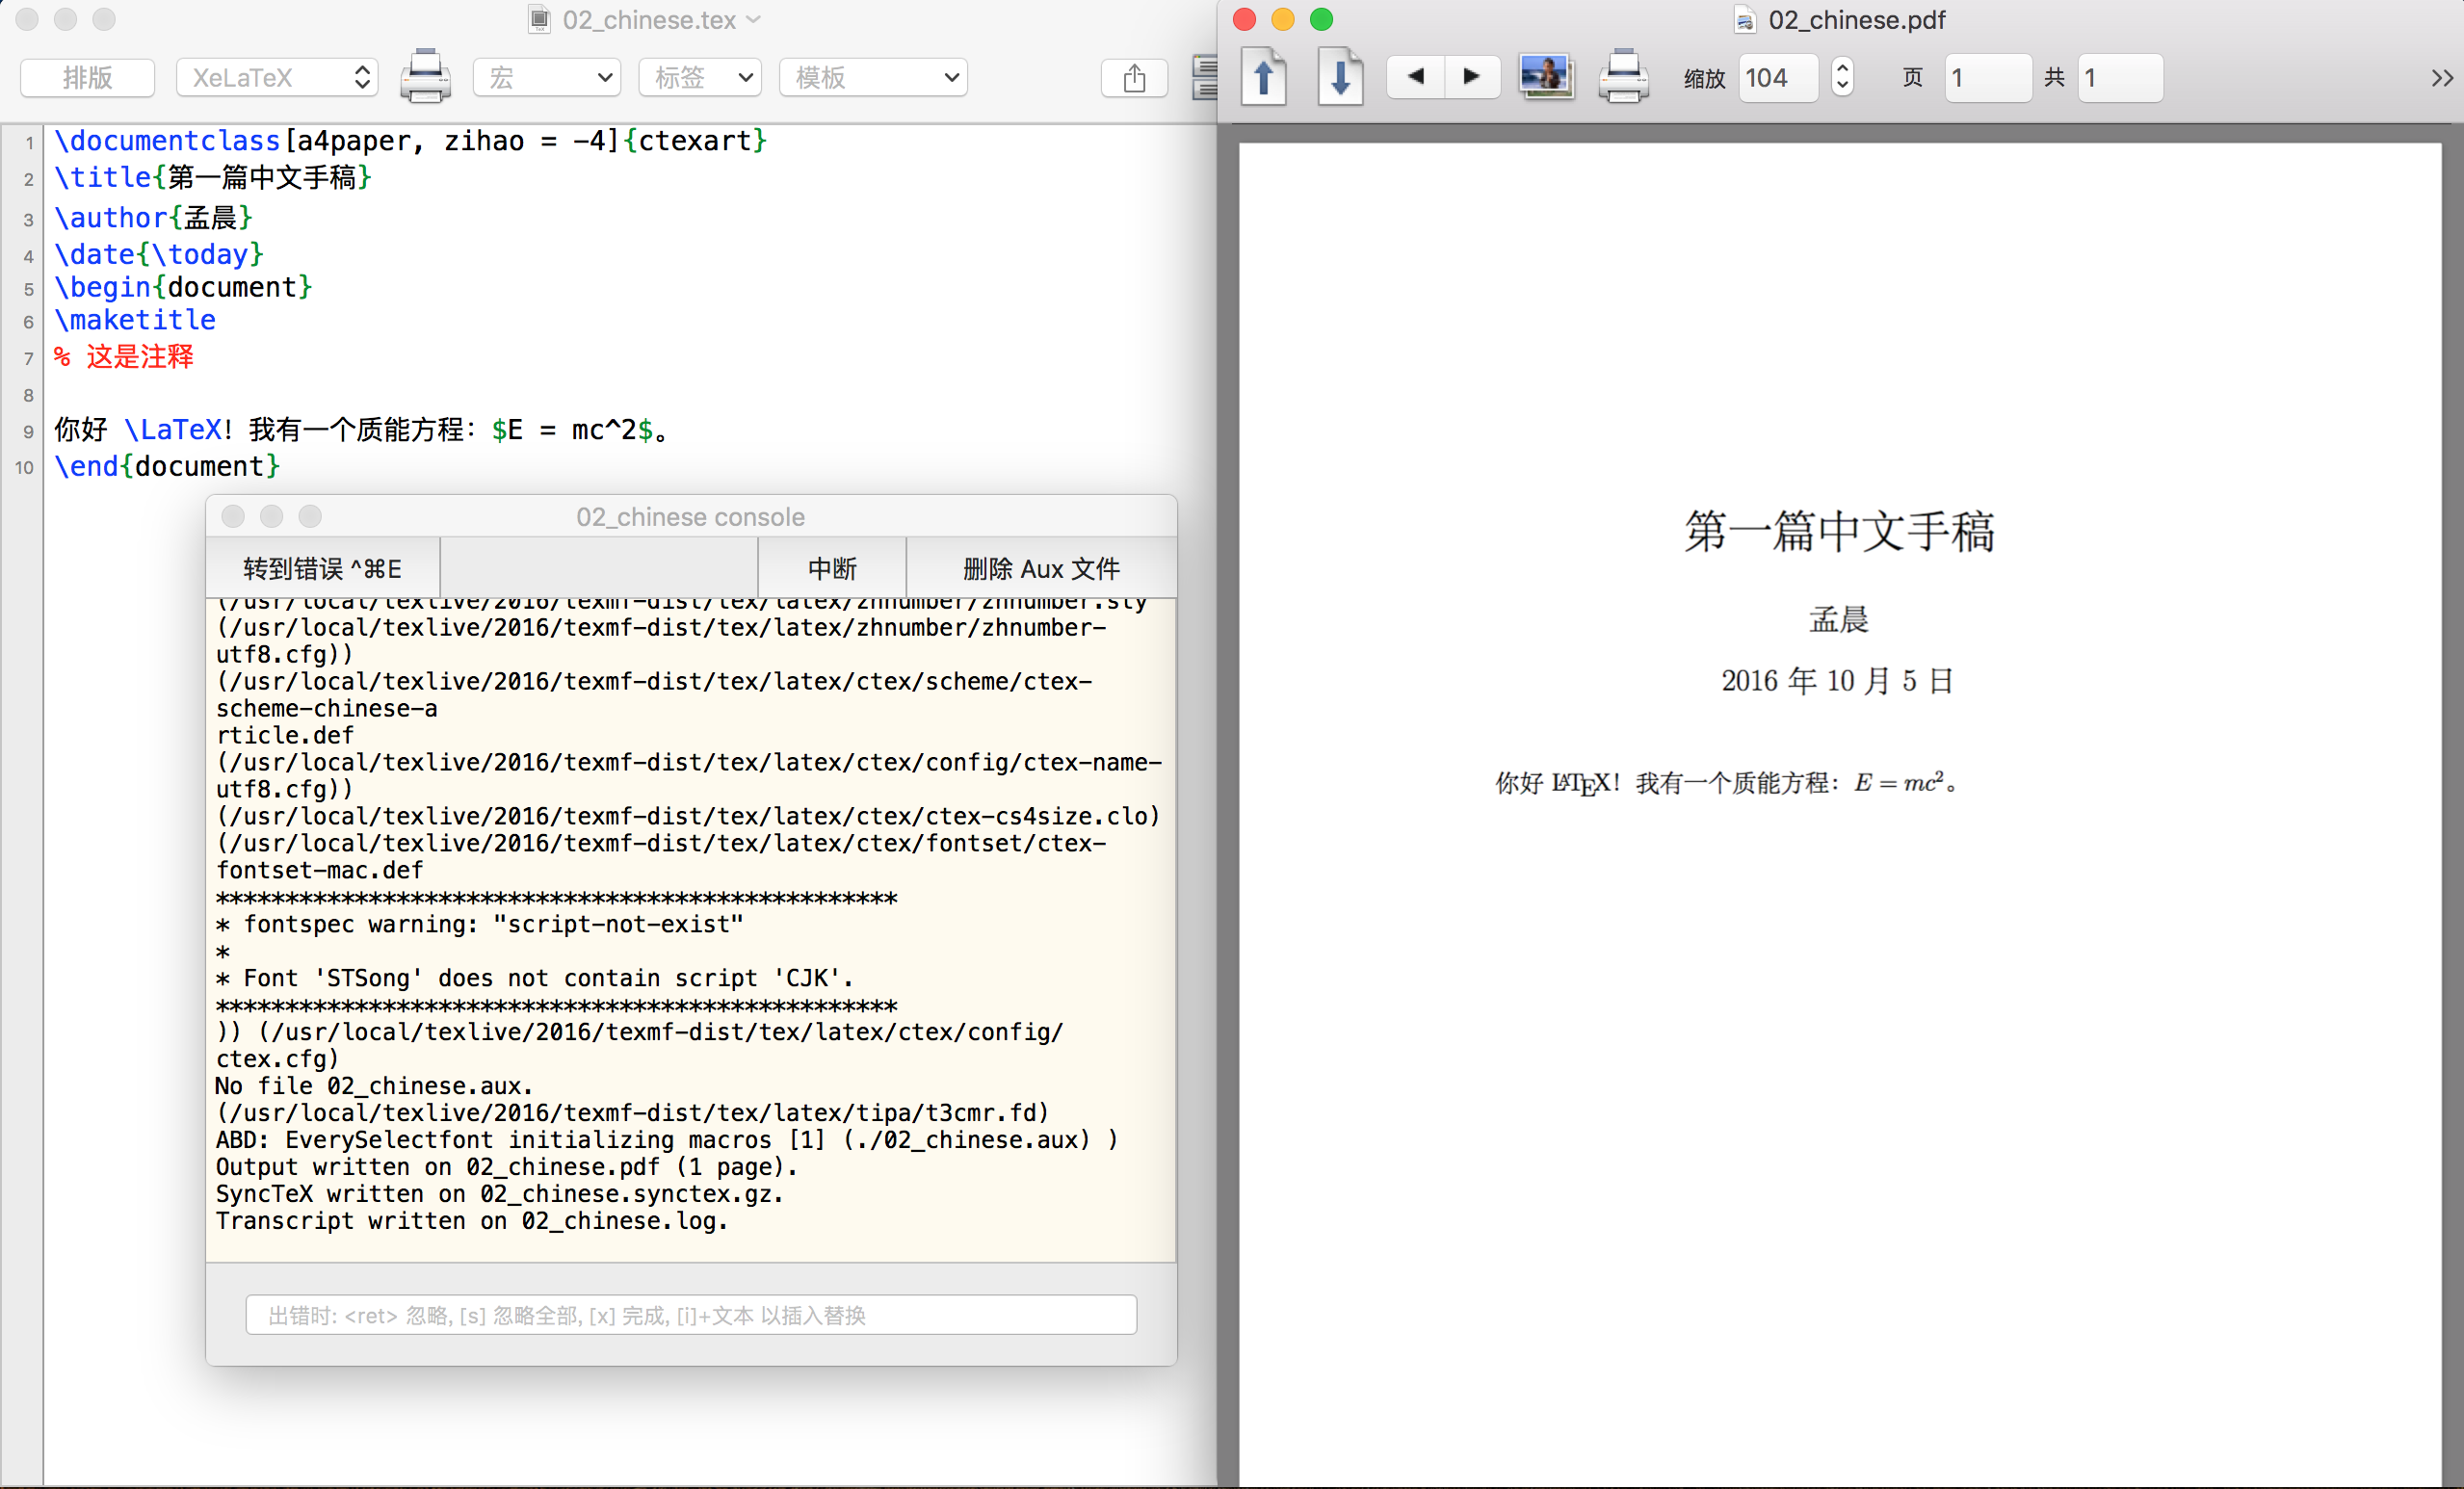
\includegraphics[width = .8\linewidth]{02_chinese_mac.png}
\caption{你好 \LaTeX{}}\label{fig:chinese}
\end{figure}

从此开始,我就不把每次编译的代码、编译窗口和结果一并截图上来了,也不会区分操作系统的版本。
我只会贴出正确的输出结果。
实际上,你应该逐渐养成习惯,明白什么样的代码会打印出什么内容。

\section{额外习题}

你需要完成这些额外习题,帮助你巩固学到的知识。如果你觉得这部分习题很难,可以先看后面的内容——
但一定要记着回来,解决这些问题。

\begin{enumerate}
  \item 使用 \lstinline[style = iltx]|ctexbook| 和
  \lstinline[style = iltx]|ctexrep| 替换 \lstinline[style = iltx]|article|,
  看看会有什么效果。使用搜索引擎,检索相关资料。
  \item 阅读 \ctex{} 宏集的说明书(方法是在命令行中执行
  \lstinline[style = ibash]|texdoc ctex|),了解如果希望%
  \emph{只提供中文支持,不改变版式}应该怎样做。
  \item 尝试打印出这些特殊符号:\#, \$, \textbackslash, \{, \}, \_, \^{}。
  使用搜索引擎,检索\emph{转义符}的相关知识,了解 \LaTeX{} 有哪些符号需要转义才能打印出来。
\end{enumerate}

\endinput
